%-------------------------------------------------------------------------------
%
% pre-Header
%
%
%-------------------------------------------------------------------------------
\documentclass[english]{article}
\usepackage[T1]{fontenc}
\usepackage[latin1]{inputenc}
\usepackage{graphicx}
\usepackage{amssymb}
\usepackage{amsmath}
\usepackage{times}
\usepackage{geometry}
\usepackage{color}
\usepackage{multirow}
\usepackage{bigstrut}

\geometry{verbose,letterpaper,tmargin=1in,bmargin=1in,lmargin=1in,rmargin=1in}
\DeclareMathOperator*{\avg}{average}
\usepackage{babel}

\begin{document}
\newtheorem{thm}{Theorem}
\newtheorem{cor}{Corollary}
\newtheorem{argm}{Argument}
\newtheorem{defn}{Definition}
\newtheorem{theorem}{Theorem}[section]
\newtheorem{lemma}[theorem]{Lemma}
\newtheorem{proposition}[theorem]{Proposition}
\newtheorem{corollary}[theorem]{Corollary}
\newenvironment{proof}[1][Proof]{\begin{trivlist}
\item[\hskip \labelsep {\bfseries #1}]}{\end{trivlist}}
\newenvironment{definition}[1][Definition]{\begin{trivlist}
\item[\hskip \labelsep {\bfseries #1}]}{\end{trivlist}}
\newenvironment{example}[1][Example]{\begin{trivlist}
\item[\hskip \labelsep {\bfseries #1}]}{\end{trivlist}}
\newenvironment{remark}[1][Remark]{\begin{trivlist}
\item[\hskip \labelsep {\bfseries #1}]}{\end{trivlist}}
\newcommand{\qed}{\nobreak \ifvmode \relax \else
\ifdim\lastskip<1.5em \hskip-\lastskip
\hskip1.5em plus0em minus0.5em \fi \nobreak
\vrule height0.75em width0.5em depth0.25em\fi}

\newcommand{\etal}{\textit{et al. }}
\newcommand{\TT}{\times 10^}

%-------------------------------------------------------------------------------
%
% Title
%
%-------------------------------------------------------------------------------
\title{A Second Order Accurate Level Set Method on Non-Graded Adaptive Cartesian Grids}
\author{Chohong Min \thanks{Mathematics Department, University of California, Santa Barbara, CA 93106.} \hspace{2cm}
Fr\'{e}d\'{e}ric Gibou \thanks{Mechanical Engineering Department \& Computer Science Department,
University of California, Santa Barbara, CA 93106.}} \maketitle
\begin{abstract}
We present a level set method on non-graded adaptive Cartesian grids, i.e.
grids for which the ratio between adjacent cells is not constrained. We use
quadtree and octree data structures to represent the grid and a simple
algorithm to generate a mesh with the finest resolution at the interface.
In particular, we present (1) a locally third order accurate
reinitialization scheme that transforms an arbitrary level set function
into a signed distance function, (2) a second order accurate
semi-Lagrangian methods to evolve the linear level set advection equation
under an externally generated velocity field, (3) a second order accurate
upwind method to evolve the nonlinear level set equation under a normal
velocity as well as to extrapolate scalar quantities across an interface in
the normal direction, and (4) a semi-implicit scheme to evolve the
interface under mean curvature. Combined, we obtain a level set method on
adaptive Cartesian grids with a negligible amount of mass loss. We propose
numerical examples in two and three spatial dimensions to demonstrate the
accuracy of the method.
\end{abstract}


%-------------------------------------------------------------------------------
%
% Introduction
%
%-------------------------------------------------------------------------------
\section{Introduction}

Many problems in science and engineering can be described by a moving free
boundary model. Examples include free surface flows, Stefan problems and
multiphase flows to cite a few. The difficulty in solving these problems
stems from the fact that: First, they involve dissimilar length scales.
Second, the boundary position must be computed as part of the solution
process. Third, the interface may be expected to undergo complex
topological changes, such as the merging or the pinching of two fronts.
Numerically, the interface that separates the two phases can be either
explicitly tracked or implicitly captured. Several classes of successful
methods exist with their own virtues and drawbacks.

Volume of Fluid methods
\cite{benson:1992:hydrocodes,benson:2002:VOF_Review,DeBar:1974:KRAKEN,Hirt_Nichols:1981:VOF,Noh_Woodward:1976:SLIC,Youngs:1984:VOF}
have the advantage of being volume preserving since the mass fraction in
each cell is being tracked. However, it is often difficult to extract
geometrical properties such as curvatures due to the fact that it is
challenging or even impossible to reconstruct a smooth enough function from
the mass fractions alone. We note however that some recent improvement in
interface reconstruction can be found in \cite{Dyadechko:2006:MOF}.

The main advantage of an explicit approach, e.g. front tracking
\cite{glimm:1999:fronttracking, Juric:1996:Dendritic_Solidification,
Juric:1998:Boiling_Flows, Tryggvason:2001:Front_Tracking_Flows_Review}, is
its accuracy. The main disadvantage is that additional treatments are
needed for handling changes in the interface's topology. In turn, the
explicit treatment of connectivity makes the method challenging to extend
to three spatial dimensions. While researchers have produced remarkable
results for a wide variety of applications using front tracking techniques,
these difficulties make this approach not ideally suited for studying
interface problems with changes in topology. Implicit representations such
as the level set method or the phase-field method represent the front as an
isocontour of a continuous function. Topological changes are consequently
handled in a straightforward fashion, and thus these methods are readily
implemented in both two and three spatial dimensions.

The main idea behind the phase-field method is to distinguish between
phases with an order parameter (or phase-field) that is constant within
each phase but varies smoothly across an interfacial region of finite
thickness. The dynamics of the phase-field is then coupled to that of the
solution in such a way that it tracks the interface motion and approximates
the sharp interface limit when the order parameter vanishes. Phase-field
methods are very popular techniques for simulating dendritic growth for
example and have produced accurate quantitative results, e.g.
\cite{Langer:1986:Phase_Field, Karma_Rappel:1997:Phase_Field_2D_3D,
Karma:2001:Phase_Field_Different_Diffusion,
Nestler:2005:Phase_Field_FEM_FDM, Schmidt:1996:CTD}. However, these methods
suffer from their own limitations: Phase-field methods have only an
approximate representation of the front location and thus the
discretization of the diffusion field is less accurate near the front,
resembling an enthalpy method \cite{chorin:1967:ANM}. Another consequence
is the stringent time step restriction imposed by such methods. Karma and
Rappel \cite{Karma_Rappel:1996:Phase_Field_Kinetics} have developed a
thin-interface limit of the phase-field model with a significant
improvement of the capillary length to interface thickness ratio
constraint; however, the time step restriction is still on the order of the
microscopic capillary length. Another disadvantage is the potential
difficulty in relating the phase-field parameters to the physical
parameters \cite{Wheeler:1993:Handbook}, although some progress is being
made for some wider class of problems
\cite{Elder_Provatas:2001:Phase_Field_Sharp_Interface}.

The main difference between the phase-field method and the level set approach
\cite{osher:1988:originallevelset, sethian:1999:levelset, osher:2002:levelset} is that the level
set method is a sharp interface model. The level set can therefore be used to exactly locate the
interface in order to apply discretizations that depend on the exact interface location.
Consequently, the sharp interface equation can be solved directly with no need for asymptotic
analysis, which makes the method potentially more attractive in developing general tool box
software for a wide range of applications. Another advantage is that only the standard time step
restrictions for stability and consistency are required, making the method significantly more
efficient. Level set methods have been extremely successful on uniform grids in the study of
physical problems such as compressible flows, incompressible flows, multiphase flows (see e.g.
\cite{osher:2002:levelset, sethian:1999:levelset} and the references therein), Epitaxial growth
(see e.g.\cite{Caflisch:1999:Island_Dynamics, Gibou:2001:Rate_Equations_Scaling_Laws,
Gibou:2001:Rate_Equations, Ratsch:2001:Island_Dynamics_Review} and the references therein) or in
image processing (see e.g. \cite{osher:2003:levelset} and the references therein). One of the main
problem of the level set method, namely its mass loss, has been partially solved with the advent of
the particle level set method of Enright \etal \cite{Enright:2002:PLS}. Within this method, the
interface is captured by the level set method and massless particles are added in order to reduce
the mass loss. The massless particles are also used in the reinitialization process for obtaining
smoother results for the reinitialized level set function. However, the use of particles adds to
the CPU and the memory requirement and cannot be applied for flows producing shocks. Rather
recently, there has been a thrust in developing level set methods on adaptive Cartesian grids. For
example Losasso \etal \cite{losasso:2004:octree} presented a particle level set based method to
simulate free surface flows on non-graded Cartesian grids. Within this method, the interface
between the liquid and the air is captured by the particle level set on a non graded octree data
structure. Other interesting work on adaptive level-set methods can be found in
\cite{droske01adaptive} and \cite{Milne:1995:thesis}.

In this paper, we present a general particle-less level set method on
non-graded Cartesian grids that produces a negligible amount of mass loss.
We apply this method to the level set evolution (1) with an externally
generated velocity field, (2) in the normal direction and (3) under mean
curvature. We also present a locally third order accurate reinitialization
scheme that transforms an arbitrary function into a sign distance function
as well as standard techniques to extrapolate a scalar quantities across an
interface in its normal direction.

\section{The Level Set Method}
The level set method, introduced by Osher and Sethian
\cite{osher:1988:originallevelset} describes a curve in two spatial
dimensions or a surface in three spatial dimensions by the zero-contour of
a higher dimensional function $\phi$, called the level set function. For
example, in two spatial dimension, a curve is define by $\{(x, y):
\phi(x,y)=0\}$. Under a velocity field $V$, the interface deforms according
to the level set equation
\begin{eqnarray}
\phi_t+V \cdot \nabla \phi = 0. \label{eq_levelset}
\end{eqnarray}
To keep the values of $ \phi $ close to those of a signed distance
function, i.e. $ |\nabla \phi| = 1 $, the reinitialization equation
introduced in Sussman \etal \cite{Sussman:1994:levelsetincompressible}
\begin{eqnarray}
\phi_{\tau} + S(\phi_o) \left( |\nabla \phi| - 1 \right) =0 \label{reinit}
\end{eqnarray}
is traditionally iterated for a few steps in fictitious time, $ \tau $.
Here $S(\phi_o)$ is a smoothed out sign function. The level set function is
used to compute the normal $$ \vec{n} = \nabla \phi/|\nabla \phi|, $$ and
the mean curvature $$\kappa = \nabla \cdot \vec{n}. $$ We refer the
interested readers to the book by Osher and Fedkiw
\cite{osher:2002:levelset} as well to the book by Sethian
\cite{sethian:1999:levelset} for more details on the level set method.

%-------------------------------------------------------------------------------
%
% Spatial Discretization
%
%-------------------------------------------------------------------------------
\section{Spatial Discretization and Refinement Criterion \label{sec_spatial_discretization}}

We use a standard quadtree (resp. octree) data structure to represent the
spatial discretization of the physical domain in two (resp. three) spatial
dimensions as depicted in figure \ref{fig_quadtree_description}: Initially
the root of the tree is associated with the entire domain, then we
recursively split each cell into four children until the desired level of
detail is achieved. This is done similarly in three spatial dimensions,
except that cells are split into eight cubes (children). We refer the
reader to the books of Samet \cite{Samet:1990:AOS,Samet:1989:TDA} for more
details on quadtree/octree data structures.

By definition, the difference of level between a parent cell and its direct
descendant is one. The level is then incremented by one for each new
generation of children.  A tree in which the difference of level between
adjacent cells is at most one is called a graded tree. Meshes associated
with graded trees are often used in the case of finite element methods in
order to produce procedures that are easier to implement. Graded Cartesian
grids are also used in the case of finite difference schemes, see for
example the work of Popinet \cite{Popinet:2003:Gerris} for the study of
incompressible flows. Graded meshes impose that extra grid cells must be
added in regions where they are not necessarily needed, consuming some
computational resources that cannot be spent elsewhere, eventually limiting
the highest level of detail that can be achieved. Moore
\cite{Moore:1995:The_Cost_of_Balancing_Quadtrees} demonstrates that the
cost of transforming an arbitrary quadtree into a graded quadtree could
involve 8 times as many grid nodes. Weiser \cite{Weiser:1981:thesis}
proposed a rough estimate for the three dimensional case and concluded that
as much as 71 times as many grid nodes could be needed for balancing
octrees. These estimates clearly represent the worse case scenarios that
seldom exist in practical simulations. However, there is still a non
negligible difference between graded and non graded grids. In addition, not
imposing any constraint on the difference of level between two adjacent
cells allows for easier/faster adaptive mesh generations.

\begin{figure}
\begin{center}\includegraphics[scale=0.3]{quadtree_description.eps}
\includegraphics[scale=0.3]{quadtree_description_2.eps}\end{center}
\caption{Discretization of a two dimensional domain (left) and its quadtree
representation (right). The entire domain corresponds to the root of the
tree (level 0). Then each cell can be recursively subdivided further into
four children. In this example, the tree is ungraded since the difference
of level between cells exceeds one.\label{fig_quadtree_description}}
\end{figure}

In this work we choose to impose that the finest cells lie on the
interface, since it is the region of interest for the level set method. In
order to generate adaptive Cartesian grids, one can use the signed distance
function to the interface along with the Whitney decomposition, as first
proposed by Strain in \cite{strain:1999:tree}. Simply stated, one
\textit{"splits any cell whose edge length exceeds its distance to the
interface"}. For a general function $\phi:\mathbb{R}^n\to\mathbb{R}$ with
Lipschitz constant $Lip(\phi)$, the Whitney decomposition was extended in
Min \cite{min:2004:lls}: Starting from a root cell split any cell $C$ if
$$\min_{v\in \textrm{vertices}(C)}|\phi(v)| \le \textrm{Lip}(\phi)\cdot
\textrm{diag-size}(C),$$ where diag-size($C$) refers to the length of the
diagonal of the current cell $C$ and $v$ refers to a vertex (node) of the
current cell.

%-------------------------------------------------------------------------------
%
% T-junction Nodes
%
%-------------------------------------------------------------------------------
\section{Finite Difference Discretizations\label{sec_finite_differences}}
\begin{figure}
\begin{center}\includegraphics[scale=0.45]{neighbors_of_node_quadtree.eps}
\end{center}
\caption{Neighboring nodes of a T-junction node,
$v_0$.\label{fig_T_junction_quadtree}}
\end{figure}

In the case of non regular Cartesian grids, the main difficulty comes from
deriving discretizations at T-junction nodes, i.e. nodes for which there is
a missing neighboring node in one of the Cartesian directions. For example
figure \ref{fig_T_junction_quadtree} depicts a T-junction node $v_0$, with
three neighboring nodes $v_1$, $v_2$ and $v_3$ aligned in the Cartesian
directions and one ghost neighboring node $v_4$ replacing the missing grid
node in the positive Cartesian direction. The value of a node-sampled
function $\phi:\{v_i\}\to\mathbb{R}$ at the ghost node $v_4$ could for
example be define by linear interpolation:
\begin{equation}
\phi_4^G = \frac{\phi_5 s_6+\phi_6 s_5}{s_5+s_6}. \label{eq_bilinear_interpolation_ghost_node_in_quadtree}
\end{equation}
However, instead of using this second order accurate interpolation, one can
instead use the following third order accurate interpolation: First, note
that a simple Taylor expansion demonstrates that the interpolation error in
equation \ref{eq_bilinear_interpolation_ghost_node_in_quadtree} is given
by:
\begin{equation}
\phi_4^G = \frac{\phi_5 s_6+\phi_6
s_5}{s_5+s_6}=\phi(v_4)+\frac{s_5s_6}{2}\phi_{yy}(v_0) + O(\triangle
x_{\textrm{smallest}})^3, \label{Taylor_Quadtree}
\end{equation}
where $\triangle x_{\textrm{smallest}}$ is the size of the smallest grid
cell with vertex $v_0$. The term $\phi_{yy}(v_0)$ can be approximated using
the standard first order accurate discretization
$\frac{2}{s_2+s_3}\left(\frac{\phi_2-\phi_0}{s_2}
+\frac{\phi_3-\phi_0}{s_3}\right)$ and cancelled out in equation
\ref{Taylor_Quadtree} to give:
\begin{equation}
\phi_4^G = \frac{\phi_5 s_6+\phi_6 s_5}{s_5+s_6}-\frac{s_5s_6}{s_2+s_3}\left(\frac{\phi_2-\phi_0}{s_2} +\frac{\phi_3-\phi_0}{s_3}\right). \label{eq_quadratic_interpolation_ghost_node_in_quadtree}
\end{equation}
We also point out that this interpolation only uses the node values of the
cells adjacent to $v_0$, which is particularly beneficial since access to
cells not immediately adjacent to the current cell is more difficult and
could add on CPU time and/or memory requirement.


\begin{figure}
\begin{center}\includegraphics[
  scale=0.45]{neighbors_of_node_octree.eps}
\end{center}
\caption{Neighboring vertices of a vertex three spatial
dimensions.\label{fig_T_junction_octree}}
\end{figure}

In three spatial dimensions, similar interpolation procedures can be used
to define the value of $\phi$ at ghost nodes. Referring to figure
\ref{fig_T_junction_octree}, a T-junction node $v_0$ has four regular
neighboring nodes and two ghost nodes. The values of a node-sampled
function $\phi:\{v_i\}\to\mathbb{R}$ at the ghost nodes $v_4$ and $v_5$ can
be defined by second order linear and bilinear interpolations as:
\begin{equation}
\begin{split}
\phi_4^G &= \frac{s_7\phi_8+s_8\phi_7}{s_7+s_8}, \\
\phi_5^G &= \frac{ s_{11}s_{12}\phi_{11}+ s_{11}s_{ 9}\phi_{12}+
s_{10}s_{12}\phi_{ 9}+ s_{10}s_{9}\phi_{10} }
{(s_{10}+s_{11})(s_{9}+s_{12})}.
\end{split}
\label{eq_linear_interpolation_ghost_node_in_octree}
\end{equation}
As in the case of quadtrees, third order accurate interpolations can be
derived by cancelling out the second order derivatives in the error term to
arrive at:
\begin{equation}
\begin{split}
\phi_4^G &= \frac{s_7\phi_8+s_8\phi_7}{s_7+s_8}
           - \frac{s_7s_8}{s_3+s_6}
            \left( \frac{\phi_3-\phi_0}{s_3} +
                   \frac{\phi_6-\phi_0}{s_6}
            \right), \\
\phi_5^G &= \frac{
s_{11}s_{12}\phi_{11}+
s_{11}s_{ 9}\phi_{12}+
s_{10}s_{12}\phi_{ 9}+
s_{10}s_{9}\phi_{10}
}{(s_{10}+s_{11})(s_{9}+s_{12})} \\
          &\quad - \frac{s_{10}s_{11}}{s_3+s_6}
            \left( \frac{\phi_3-\phi_0}{s_3} +
                   \frac{\phi_6-\phi_0}{s_6}
            \right) \\
          &\quad - \frac{s_{9}s_{12}}{s_1+s_4}
            \left( \frac{\phi_1-\phi_0}{s_1} +
                   \frac{\phi_4^G-\phi_0}{s_4}
            \right).
\end{split}
\label{eq_quadratic_interpolation_ghost_node_in_octree}
\end{equation}
We emphasize that figure \ref{fig_T_junction_octree} represents the general
configuration of neighboring nodes in the case of an octree as described in
Min \etal \cite{Min::Poisson_AMR_Second_Order}.

The third order interpolations defined above allow us to treat T-junction
nodes in a same fashion as a regular node, up to third order accuracy.
Here, we refer to a regular node as a node for which all the neighboring
nodes in the Cartesian directions exist. Therefore, we can then define
finite differences for $\phi_x$, $\phi_y$, $\phi_z$, $\phi_{xx}$,
$\phi_{yy}$ and $\phi_{zz}$ at every nodes using standard finite difference
formulas in a dimension by dimension framework. For example, refering to
figure \ref{fig_one_dimensional_adaptive_grid}, we use the standard
discretization for $\phi_x$ and $\phi_{xx}$, namely the central difference
formulas:
\begin{equation}
\begin{split}D^0_x\phi_0=\frac{\phi_2-\phi_0}{s_2}\cdot\frac{s_1}{s_1+s_2} + \frac{\phi_0-\phi_1}{s_1}\cdot\frac{s_2}{s_1+s_2},\\
D^0_{xx}\phi_0=\frac{\phi_2-\phi_0}{s_2}\cdot\frac{2}{s_1+s_2} - \frac{\phi_0-\phi_1}{s_1}\cdot\frac{2}{s_1+s_2},
\end{split}
\label{Central_Differencing}
\end{equation}
the forward and backward first order accurate approximations of the first order derivatives:
\begin{equation}
\begin{split}
D^+_x\phi_0 &= \frac{\phi_2-\phi_0}{s_2},\\
D^-_x\phi_0 &= \frac{\phi_0-\phi_1}{s_1},
\end{split}
\label{one_sided_1_fdm}
\end{equation}
and the second order accurate approximations of the first order derivatives:
\begin{equation}
\begin{split}
D^+_x\phi_0 &= \frac{\phi_2-\phi_0}{s_2} - \frac{s_2}{2}\text{minmod}\left(D^0_{xx}\phi_0,D^0_{xx}\phi_2\right),\\
D^-_x\phi_0 &= \frac{\phi_0-\phi_1}{s_1} +
\frac{s_1}{2}\text{minmod}\left(D^0_{xx}\phi_0,D^0_{xx}\phi_1\right),
\end{split}
\label{one_sided_2_fdm}
\end{equation}
where we use the minmod slope limiter \cite{Shu:1988:ENO,liu:1996:WENO}
because it produces more stable results in region where $\phi$ might
present kinks. Similarly, approximations for first and second order
derivatives are obtained in the $y$ and $z$ directions.

\begin{figure}
\begin{center}
\includegraphics[scale=0.9]{one_dimensional_adaptive_grid.eps}
\end{center}
\caption{One dimensional adaptive grid}
\label{fig_one_dimensional_adaptive_grid}
\end{figure}
%-------------------------------------------------------------------------------
%
% Interpolations
%
%-------------------------------------------------------------------------------
\section{Interpolation Procedures\label{sec_interpolation}}
Some reserve must be provided to define data anywhere in a cell, for
example in order to use semi-Lagrangian methods (see section
\ref{sec_semi_lagrangian}). As pointed out in Strain
\cite{Strain:2000:FSL}, the most natural choice of interpolation in
quadtree (resp. octree) data structures is the piecewise bilinear (resp.
trilinear) interpolation: Consider a cell $C$ with dimensions $[0, 1]^2$,
the bilinear interpolation at a point $x \in C$ using the values at the
nodes reads:
\begin{equation}
\begin{split}
\phi(x,y) &= \phi(0,0)(1-x)(1-y) \\
          &+ \phi(0,1)(1-x)(\quad\,\,\,\,\,y) \\
          &+ \phi(1,0)(\quad\,\,\,\,\,x)(1-y) \\
          &+ \phi(1,1)(\quad\,\,\,\,\,x)(\quad\,\,\,\,\,y)
\end{split}
\label{Bilinear_Interpolation}
\end{equation}
Quadratic interpolation can also easily be constructed using the data from the parent cell: Since
the parent cell of any current cell of a quadtree (resp. octree) owns $2\times 2$ children cells
(resp. $2\times 2\times 2$) and $3\times 3$ nodes (resp. $3\times 3\times 3$), one can defined the
multidimensional Lagrange quadratic interpolation on the parent cell. For example in the case of a
cell $[-1, 1]^2$ in a quadtree, we can define the Lagrange interpolation as:
\begin{equation*}
\begin{aligned}
\phi(x,y) &= \phi(\textrm{-1},\textrm{-1})\frac{x(x-1)}2\frac{y(y-1)}2 \\
          &+ \phi(\textrm{-1},\,\,      0)\frac{x(x-1)}2(y^2-1)        \\
          &+ \phi(\textrm{-1},\,\,      1)\frac{x(x-1)}2\frac{y(y+1)}2
\end{aligned}
\begin{aligned}
+ \phi(0,\textrm{-1})(x^2-1)\frac{y(y-1)}2 &+ \phi(1,\textrm{-1})\frac{x(x+1)}2\frac{y(y-1)}2 \\
+ \phi(0,\,\,      0)(x^2-1)(y^2-1)        &+ \phi(1,\,\,     0)\frac{x(x+1)}2(y^2-1)        \\
+ \phi(0,\,\,      1)(x^2-1)\frac{y(y+1)}2 &+ \phi(1,\,\,
1)\frac{x(x+1)}2\frac{y(y+1)}2.
\end{aligned}
\end{equation*}
However, this interpolation procedure is sensitive to nearby
discontinuities, e.g. near kinks. We therefore prefer to define a quadratic
interpolation by correcting equation (\ref{Bilinear_Interpolation}) using
second order derivatives. For a cell $[0, 1]^2$, we have:
\begin{equation}
\begin{aligned}
\phi(x,y) &= \phi(0,0)(1-x)(1-y) \\
          &+ \phi(0,1)(1-x)(\quad\,\,\,\,\,y) \\
          &+ \phi(1,0)(\quad\,\,\,\,\,x)(1-y) \\
          &+ \phi(1,1)(\quad\,\,\,\,\,x)(\quad\,\,\,\,\,y)
\end{aligned}
\begin{aligned}
\\
\\
\\        &- \phi_{xx}\frac{x(1-x)}2
           - \phi_{yy}\frac{y(1-y)}2,
\end{aligned}\label{Stabilized_Interpolation1}
\end{equation}
where we define
\begin{equation}
\begin{aligned}
\phi_{xx}&=\min_{v\in \textrm{vertices}(C)}(|D^0_{xx}\phi_{v}|),\\
\phi_{yy}&=\min_{v\in \textrm{vertices}(C)}(|D^0_{yy}\phi_{v}|).
\end{aligned}\label{Stabilized_Interpolation2}
\end{equation}
Since a distant function is piecewise differentiable in general, the choice of the smallest in
absolute value enhances the numerical stability of the interpolation.


%-------------------------------------------------------------------------------
%
% Reinitialization
%
%-------------------------------------------------------------------------------
\section{Reinitialization Scheme\label{sec_reinitialization}}
In principle, the level function can be chosen as any Lipschitz continuous function. However, the
so-called signed distance function is known to produce more robust numerical results, to improve
mass conservation and to reduce errors in the computations of geometrical quantities such as the
interface curvatures. Sussman \etal proposed in \cite{sussmanfatemi:1998:redistancing} to evolve
the following partial differential equation to steady state in order to reinitialize a level set
function $\phi^0:\mathbb{R}^n\to\mathbb{R}$ into the signed distance function $\phi$:
\begin{equation}
\phi_{\tau} + \mathrm{sgn}(\phi^0)\left( |\nabla\phi|-1 \right)=0,
\label{eq_reinitialization}
\end{equation}
where $\tau$ represents the fictitious time. A standard discretization for
this equation in its semi-discrete form is given by:
\begin{equation}\frac{d\phi}{d\tau} + \mathrm{sgn}(\phi^0)
\left[ H_G\left(D_x^+\phi, D_x^-\phi,
                D_y^+\phi, D_y^-\phi\right)-1\right]=0,\label{Semi_Discrete}\end{equation}
where $\mathrm{sgn}(\phi^0)$ denotes the signum of $\phi^0$ and $H_G$ is the Godunov Hamiltonian
defined as:
\begin{equation*}
H_G(a,b,c,d)=
\begin{cases}
\sqrt{\max(|a^+|^2,|b^-|^2)+\max(|c^+|^2,|d^-|^2)} & \textrm{ if }
\mathrm{sgn}(\phi^0)\le 0 \\
\sqrt{\max(|a^-|^2,|b^+|^2)+\max(|c^-|^2,|d^+|^2)} & \textrm{ if } \mathrm{sgn}(\phi^0)>0
\end{cases},
\end{equation*}
with $a^+=\max(a,0)$ and $a^-=\min(a,0)$. The one-sided derivatives,
$D_x^{\pm}\phi$ and $D_y^{\pm}\phi$ are discretized by the second order
accurate one-sided finite differences defined in section
\ref{sec_finite_differences}. Equation (\ref{Semi_Discrete}) is evolved in
time with the TVD RK-2 method given in Shu and Osher \cite{Shu:1988:ENO}:
First define $\tilde{\phi}^{n+1}$ and $\tilde{\phi}^{n+2}$ by Euler steps
\begin{eqnarray*}
\frac{\tilde{\phi}^{n+1}-\phi^n}{\triangle \tau} &+& \mathrm{sgn}(\phi^0) \left[
H_G\left(D_x^+\phi^n, D_x^-\phi^n,
                D_y^+\phi^n, D_y^-\phi^n\right)-1\right]=0,\\
\frac{\tilde{\phi}^{n+2}-\tilde{\phi}^{n+1}}{\triangle \tau} &+& \mathrm{sgn}(\phi^0) \left[
H_G\left(D_x^+\tilde{\phi}^{n+1}, D_x^-\tilde{\phi}^{n+1},
                D_y^+\tilde{\phi}^{n+1}, D_y^-\tilde{\phi}^{n+1}\right)-1\right]=0,
\end{eqnarray*} and then define $\phi^{n+1}$ by averaging:
\begin{eqnarray*}
\phi^{n+1} &=& \frac{\phi^n + \tilde{\phi}^{n+2}}2.
\end{eqnarray*}

In order to preserve area/volume, the reinitialization procedure is
required not to move the original interface defined by $\phi_0$. In their
seminal work, Russo and Smereka \cite{Russo_Smereka} solved this problem by
simply including the initial interface location (given by $\phi_0$) in the
stencils of the one-sided derivatives. Consider the case depicted by figure
\ref{fig_one_dimensional_adaptive_grid} and suppose that
$\phi^0_0\cdot\phi^0_2<0$, i.e. the interface is located between the nodes
$v_0$ and $v_2$. The interface location $v_I$ can be calculated by finding
the root of the quadratic interpolation of $\phi^0$ on the interval
$\overline{v_0v_2}$ with the origin at the center of the interval:
\begin{equation*}
\phi^0(x)=c_2x^2+c_1x+c_2,
\text{  with }
\begin{cases}
c_2 &= \frac12\text{minmod}\left[D^0_{xx}\phi^0_0,D^0_{xx}\phi^0_2\right] \\
c_1 &= (\phi^0_2-\phi^0_0)/s_2 \\
c_0 &= (\phi^0_2+\phi^0_0)/  2 - c_2s_2^2/4
\end{cases}.
\end{equation*}
The distance $s_I$ between $v_0$ and the interface location is then defined by:
\begin{equation*}
s_I = \frac{s_2}2 +
\begin{cases}
-c_0/c_1                            & \text{ if $|c_2|<  \epsilon$ }\\
(-c_1+\sqrt{c_1^2-4c_2c_0})/(2c_2)  & \text{ if $|c_2|\ge\epsilon$ and $\phi^0_0<0$}\\
(-c_1-\sqrt{c_1^2-4c_2c_0})/(2c_2)  & \text{ if $|c_2|\ge\epsilon$ and $\phi^0_0>0$}
\end{cases}.
\end{equation*}
The calculation of $D_x^+\phi^n_0$ is then modified using the interface
location and the fact that $\phi=0$ at the interface:
\begin{equation*}
D^+_x\phi^n_0 = \frac{0-\phi_0^n}{s_I} -
\frac{s_I}{2}\text{minmod}\left(D^0_{xx}\phi^n_0,D^0_{xx}\phi^n_2\right).
\end{equation*}
We note that in the original work of Russo and Smereka
\cite{Russo_Smereka}, a cubic interpolation was employed to locate the
interface, but that the above quadratic interpolation with the minmod
operator acting on the second order derivatives proved to be more stable in
the case where the level set function presents a kink nearby. We also point
out that in the original work of \cite{Russo_Smereka}, the first order
derivative $D^+_x\phi^n_0$ was discretized as:
\begin{equation*}
D^+_x\phi^n_0 = \frac{0-\phi_0^n}{s_I} -
\frac{s_I}{2}\text{minmod}\left(D^0_{xx}\phi^n_0,D^0_{xx}\phi^n_I\right),
\end{equation*}
thus included $v_I$ in the discretization of $D^0_{xx}\phi^n_I$. However,
we found that this choice leads to unstable results when the interface is
close to grid nodes. We thus slightly changed the discretization by only
using the location of the interface in the first term in order to maintain
the location of $\phi^0$, not in the discretization of second order
derivatives. Likewise, in the case where $s_I$ is close to zero (hence
$\phi^0_0$ is close to zero) we simply set $\phi^n_0=0$ to guarantee
stability. This only introduces a negligible perturbation in the location
of the zero level set.

The same process is then applied to $D^-_x\phi$ if there is a sign change between $\phi^0_0$ and
$\phi^0_1$. The time step restriction for cells cut by the interface is then:
\begin{eqnarray}
\Delta \tau = \begin{cases}
\min(s_I,s_1,s_2)                   & \textrm{in $1D$}, \\
\min(s_I,s_1,s_2,s_3,s_4)/2         & \textrm{in $2D$}, \\
\min(s_I,s_1,s_2,s_3,s_4,s_5,s_6)/3 & \textrm{in $3D$}. \\
\end{cases}
\end{eqnarray}

\subsection{Adaptive time stepping}
We note that an adaptive time step is possible since only the steady state
of \eqref{eq_reinitialization} is sought. Since the time step restriction
is adapted for each cell, the reinitialization procedure is fast: small
cells with a stringent time step restriction are located near the interface
and therefore only a few iterations are required to reach the steady state
at those cells (characteristic information flow away \textit{from} the
interface); cells far away from the interface are large and therefore do
not require a small time step restriction. For example, consider the
example depicted in figure \ref{fig_ex_reinitialization_square}, for which
the level set function is defined initially as -1 inside a square domain
(not aligned with the grid cells) and +1 outside. This initial level set
function is therefore very far from the signed distance function that we
seek to define. However, on a grid where the smallest grid has size
$dx=1/2048$, the reinitialization procedure takes only 35 iterations to
fully converge to the signed distance function in the entire domain. In
practice, the initial level set is never that far to the signed distance
function and therefore only about 5 iterations are required regardless of
the resolution of the finest level. Figure
\ref{fig_reinitialization_error_decay} illustrates the difference in the
number of iterations required between uniform time stepping and adaptive
time stepping. In the case of a uniform time step, we take $\triangle
t=\triangle x_{\text{smallest}}/2$, with $\triangle x_{\text{smallest}}$
the size of the smallest cell.

\subsection{Third order accuracy}\label{subsec_Accuracy_Reinitialization}
We also computed the convergence rates of the reinitialization algorithm
for the test problem proposed in \cite{Russo_Smereka}: Consider the level
set function initially defined as:
$$\phi^0(x,y)=\left(0.1+(x-1)^2+(y-1)^2\right)\left(\sqrt{x^2+y^2}-1\right),$$ which defines the
interface as a circle with center the origin and radius $1$. In this case, $\phi^0$ is not a signed
distance function and its gradients vary widely. Figure \ref{fig_reinitialization} illustrates the
gradual deformation of the cross-sections of $\phi^0$ as it evolves to the signed distance
function. Table \ref{tab_reinitialization} illustrates that the method is third order accurate in
the $L^1$ and $L^\infty$ norms near the interface, where we use the standard formulas for the $L^1$
and $L^\infty$ norms:
\begin{align*}
||\phi||_{\infty}=\max_{v:|\phi(v)|<1.2\Delta x}|\phi(v)-\phi_{\textrm{exact}}(v)|, \\
||\phi||_{1}=\avg_{v:|\phi(v)|<1.2\Delta x}|\phi(v)-\phi_{\textrm{exact}}(v)|, \\
\end{align*}
where $\Delta x=\Delta x_{\textrm{smallest}}$. Note that after the reinitializing the level set
function, the choice of $v:|\phi(v)|<1.2\Delta x$ ensures the selection of all the nodes adjacent
to the interface.

In the entire domain, the method is second order accurate if we keep refining all the cells. In the
practical case where only cells near the interface are refined, the accuracy in regions far away
from the interface is meaningless. In the case where the interface presents sharp corners, the
accuracy is reduced to first order in the $L^{\infty}$ norm.


%\begin{figure}[t]
%\centering
%\includegraphics[scale=0.2]{initial_phi.eps}
%\includegraphics[scale=0.2]{final_phi.eps}
%\\
%\includegraphics[scale=0.2]{initial_cross_section.eps}
%\includegraphics[scale=0.2]{final_cross_section.eps}
%\caption{Reinitialization procedure. Left: Initial level set function (top) and its zero cross
%section (bottom) defining a square domain. Right: Reinitialized level set function (top) and its
%zero cross section (bottom). In particular, the difference in the zero level set between the
%initial and final stages is negligible. In this example, the level difference between adjacent
%cells is not restricted.} \label{fig_ex_reinitialization_square}
%\end{figure}

\begin{figure}[t]
\centering
\includegraphics[scale=0.2]{losange_step.eps}
\includegraphics[scale=0.2]{losange_reinitialized.eps}
\\
\includegraphics[scale=0.2]{losange_initial.eps}
\includegraphics[scale=0.2]{losange_final.eps}
\caption{Reinitialization procedure. Left: Initial level set function (top)
and its zero cross section (bottom) defining a square domain. Right:
Reinitialized level set function (top) and its zero cross section (bottom).
In particular, the difference in the zero level set between the initial and
final stages is negligible. In this example, the level difference between
adjacent cells is not restricted.} \label{fig_ex_reinitialization_square}
\end{figure}

\begin{figure}
\begin{center}
\includegraphics[scale=1.0]{reinitialization_error_decrease.eps}
\end{center}
\caption{$L_1$ errors of the reinitialization algorithm in the case of the
adaptive time step (solid line) and the uniform time step (dotted line).}
\label{fig_reinitialization_error_decay}
\end{figure}

\begin{figure}
\begin{center}
\includegraphics[scale=0.8]{reinitialization_initial.eps}
\includegraphics[scale=0.8]{reinitialization_5_iterations.eps} \\
\includegraphics[scale=0.8]{reinitialization_10_iterations.eps}
\includegraphics[scale=0.8]{reinitialization_20_iterations.eps}
\end{center}
\caption{From top-left to bottom-right: Contours of the reinitialized level
set function of example \ref{subsec_Accuracy_Reinitialization} after 0, 5,
10 and 20 iterations. The contours are evenly plotted from -1 to 1 with a
thick line representing the zero contour.} \label{fig_reinitialization}
\end{figure}

\begin{table}
\begin{center}
\begin{tabular}{|c|c|c|c|c|c|c|c|}\hline
\multicolumn{3}{|c|}{} & \multicolumn{5}{|c|}{Finest Resolution}   \\\cline{4-8}
\multicolumn{3}{|c|}{} & $128^2$ & rate & $256^2$ & rate & $512^2$ \\\hline \multirow{4}{0.7
in}{Uniform Refinement} & \multirow{2}{*}{Near Interface}
 & $L_1     $ & $4.36\times10^{-6}$ & 2.92 & $5.77\times10^{-7}$ & 3.02 & $7.12\times10^{-8}$ \\\cline{3-8}
&& $L_\infty$ & $2.16\times10^{-5}$ & 2.74 & $3.24\times10^{-6}$ & 3.26 & $3.38\times10^{-7}$
\\\cline{2-8}
                                       & \multirow{2}{*}{Whole Domain}
 & $L_1     $ & $3.27\times10^{-4}$ & 2.14 & $7.42\times10^{-5}$ & 2.11 & $1.71\times10^{-5}$ \\\cline{3-8}
&& $L_\infty$ & $4.20\times10^{-2}$ & 1.56 & $1.43\times10^{-2}$ & 1.87 & $3.89\times10^{-3}$
\\\hline

\multirow{4}{0.7 in}{Adaptive Refinement} & \multirow{2}{*}{Near Interface}
 & $L_1     $ & $4.36\times10^{-6}$ & 2.94 & $5.70\times10^{-7}$ & 3.00 & $7.14\times10^{-8}$ \\\cline{3-8}
&& $L_\infty$ & $2.16\times10^{-5}$ & 2.87 & $2.96\times10^{-6}$ & 3.09 & $3.48\times10^{-7}$
\\\cline{2-8}
                                         & \multirow{2}{*}{Whole Domain}
 & $L_1     $ & $3.27\times10^{-4}$ & 1.06 & $1.57\times10^{-4}$ & 1.01 & $7.82\times10^{-5}$ \\\cline{3-8}
&& $L_\infty$ & $4.20\times10^{-2}$ & 0.00 & $4.20\times10^{-2}$ & 0.00 & $4.20\times10^{-3}$
\\\hline
\end{tabular}
\end{center}
\caption{Convergence rates for the reinitialization for example
\ref{subsec_Accuracy_Reinitialization}. The initial grid is shown in figure
\ref{fig_reinitialization}. The condition for a node $v_i$ to be
'\textit{near interface}' is chosen as $|\phi(v_i)|<\sqrt{2}\triangle
x_{\text{smallest}}$, where $\triangle x_{\text{smallest}}$ is the size of
the smallest cell. The '\textit{whole domain}' excludes the region near the
kink located at the origin, where accuracy drops to first order.}
\label{tab_reinitialization}
\end{table}

%-------------------------------------------------------------------------------
%
% semi-Lagrangian Method
%
%-------------------------------------------------------------------------------
%\section{Semi-Lagrangian Method\label{sec_semiL}}
%-------------------------------------------------------------------------------
%
% Moving Interface with Given Velocity
%
%-------------------------------------------------------------------------------
\section{Motion Under an Externally Generated Velocity Field}\label{sec_semi_lagrangian}
\subsection{Second Order Accurate Semi-Lagrangian Method\label{Sec_midpoint_rule}}
In the case where the velocity field is externally generated, the level set
equation \eqref{eq_levelset} is linear. In this case, one can use
semi-Lagrangian methods. Semi-Lagrangian schemes are extensions of the
Courant-Isaacson-Rees \cite{Courant:1952:CIR_Method} method for hyperbolic
equations and are unconditionally stable thus avoiding standard CFL
condition of $\Delta t \approx \Delta x_{\rm smallest}$. The general idea
behind semi-Lagrangian methods is to reconstruct the solution by
integrating numerically the equation along characteristic curves, starting
from any grid point $x_i$ and tracing back the departure point $x_d$ in the
upwind direction. Interpolation formulas are then used to recover the value
of the solution at such points. In this work, we use a second order
accurate Semi-Lagrangian method.

Consider the linear advection equation:
\begin{eqnarray}
\phi_t + U\cdot\nabla\phi&=&0, \label{Level_Set_Equation}
\end{eqnarray}
where $U$ is an externally generated velocity field. Then
$\phi^{n+1}(x^{n+1})=\phi^n(x_d)$, where $x^{n+1}$ is any grid node and
$x_d$ is the corresponding departure point from which the characteristic
curve originates. In this work, we use the second order mid-point method
for locating the departure point, as in \cite{Xiu:2001:Semi_Lagrangian_BD}:
$$ \begin{array}{rcl}
\hat{x} &=& x^{n+1} - \frac{\Delta t}2\cdot U^n(x^{n+1}), \\
x_d     &=& x^{n+1} -       \Delta t  \cdot U^{n+\frac12}(\hat{x}),
\end{array}
$$
where we define the velocity at the mid-time step $t^{n+\frac12}$ by a
linear combination of the velocities at the two previous time steps, i.e.
$U^{n+\frac12}=\frac32U^n-\frac12U^{n-1}$. Since $\hat{x}$ and $x_d$ are
not on grid nodes in general, interpolation procedures must be applied to
define $U^{n+\frac12}(\hat{x})$ and $\phi^n(x_d)$. We note that it is
enough to define $U^{n+\frac12}(\hat{x})$ with a multilinear interpolation
\eqref{Bilinear_Interpolation} and $\phi^n(x_d)$ with the quadratic
interpolation described by equations \eqref{Stabilized_Interpolation1} and
\eqref{Stabilized_Interpolation2}: Since a distance function has
discontinuities in its derivative in general, the stabilized quadratic
interpolation is preferred to the Hermite quadratic interpolation.

%-------------------------------------------------------------------------------
% Example : 2D Rotation Test
%-------------------------------------------------------------------------------
\subsection{Test: Rotation in 2D \label{ex_rotation_test_2D}}

Consider a domain $\Omega=[-1, 1]^2$ and a disk of radius $R=.15$ and center initially at $(0,
.75)$, rotating under the divergence free velocity field
$$
\begin{array}{lcr}
u(x,y) &=& -y \\
v(x,y) &=& x \\
\end{array}
$$
The final time $t=2\pi$ is the time when the rotation completes one
revolution. In the simulation, the adaptive refinement is used, and the
time step restriction is $\Delta t= 5\Delta x$. Table
\ref{tab_ex_rotation_test_2D} demonstrates second order accuracy for the
level set as well as for the mass conservation.  We note that we only
consider the grid nodes neighboring the interface in our computation of the
accuracy for the level set function $\phi$ since only those points define
the location of the interface.

\begin{table}
\begin{center}
\begin{tabular}{|c|c|c|c|c|c|c|}
\hline
Finest &$L^\infty$ error&rate&$L^1 error$&rate&Loss of&rate \\
Resolution& of $\phi$      &    & of $\phi$ &    &volume(\%)&    \\\hline
$32^2$&$7.24\times10^{-2}$&    &$3.11\times10^{-2}$&    &28.51&  \\\hline
$64^2$&$1.78\times10^{-2}$&2.02&$8.86\times10^{-3}$&1.81&7.21 & 1.98   \\\hline
$128^2$&$4.52\times10^{-3}$&1.97&$2.13\times10^{-4}$&2.05&1.78& 2.01   \\\hline
$256^2$&$1.13\times10^{-3}$&1.99&$5.56\times10^{-4}$&1.93&0.45& 1.98   \\\hline
$512^2$&$2.85\times10^{-4}$&2.00&$1.38\times10^{-4}$&2.01&0.11& 2.03   \\\hline
$1024^2$&$7.14\times10^{-5}$&2.00&$3.46\times10^{-5}$&2.00&0.03& 1.87   \\\hline
$2048^2$&$1.78\times10^{-5}$&2.00&$8.64\times10^{-6}$&2.00&0.007& 2.01   \\\hline
\end{tabular}
\end{center}
\caption{Convergence rates for example \ref{ex_rotation_test_2D}
\label{tab_ex_rotation_test_2D}}
\end{table}

%-------------------------------------------------------------------------------
% Example : Vortex Test Test
%-------------------------------------------------------------------------------
\subsection{Test: Vortex in 2D \label{ex_large_deformation_test_2D}}
In this example, we test our level set implementation on the more
challenging flow proposed by Bell \etal \cite{Bell_Colella_Glaz}: Consider
a domain $\Omega=[0, 1]^2$ and a disk of radius $.15$ and center $(.5,
.75)$ as the initial zero level set contour. The level set is then deformed
under the divergence free velocity field $U=(u,v)$ given by:
$$
\begin{array}{rcr}
u(x,y) &=& -\sin^2(\pi x)\sin(2\pi y) \\
v(x,y) &=&  \sin^2(\pi y)\sin(2\pi x) \\
\end{array}
$$
The disk is deformed forward until $t=1$ and then backward to the original
shape using the reverse velocity field with a time step restriction of
$\triangle t=5\cdot\triangle x_{\text{smallest}}$.

\begin{table}
\begin{center}
\begin{tabular}{|c|c|c|c|c|c|c|c|}\hline
\multirow{2}{*}{} & \multicolumn{7}{|c|}{Finest Resolution}   \\\cline{2-8}
                  & $64^2$ & rate & $128^2$ & rate & $256^2$ & rate & $512^2$ \\\hline
$L_1     $ error of $\phi$&$9.58\TT{-3}$&2.80&$1.38\TT{-3}$&2.02&$3.41\TT{-4}$&2.08&$8.09\TT{-5}$
\\\hline $L_\infty$ error of
$\phi$&$1.83\TT{-2}$&1.57&$6.17\TT{-3}$&1.08&$2.91\TT{-3}$&1.39&$1.11\TT{-3}$ \\\hline Volume Loss
&$4.48       $&2.36&$0.874      $&1.40&$0.331      $&1.79&$0.0954     $ \\\hline Max number of
nodes   &$1045       $&1.10&$2243       $&1.10&$4815       $&1.09&$10256      $ \\\hline Min number
of nodes   &$439        $&1.07&$924        $&0.99&$1831       $&1.01&$3679       $ \\\hline
time(sec) & 1.420 & 2.29 & 6.96 & 2.17 &31.4 & 2.13 & 138 \\
\hline minimum memory(MB) & 0.0448 & 1.07 & 0.0943 & .97 & 0.185 & 1.00 & 0.371 \\
\hline maximum memory(MB) & 0.101 & 1.30 & 0.248 & 1.06 & 0.517 & 1.03 & 1.06 \\ \hline
\end{tabular}
\end{center}
\caption{Convergence rates for example \ref{ex_large_deformation_test_2D}. The memory
requirement increases linearly with effective resolution since most of the computational resources
is focused near the one-dimensional interface, i.e. our method is an efficient implementation of
local level set methods. The computational time increases quadratically with effective resolution,
since the number of nodes is doubled and the time step is halved.} \label{tab_vortex}
\end{table}


Table \ref{tab_vortex} demonstrate second order accuracy for $L_1$ error of
$\phi$ and volume of loss, and linear increase in the maximum/minimum
number of nodes. Note that the uniform grid of resolution $512^2$ requires
about 25 times more nodes than the adaptive grid with the same resolution.
Although second order accuracy was achieved in both the maximum and average
norms in the previous example, the convergence rate of the maximum error is
oscillating between one and two. This is due to the fact that as the
interface deforms, some part of the interface are under resolved. Figure
\ref{fig_vortex_test} illustrates this at $t=1$: Here, the tail of the
interface is not resolved accurately. This deterioration in accuracy was
also reported in \cite{Olsson_Kreiss:2005}.

\begin{figure}
\begin{center}
\includegraphics[scale=0.7]{vortex_flow_at_one.eps}
\includegraphics[scale=0.7]{vortex_flow_at_two.eps}
%%includegraphics[scale=0.7]{volume_loss.eps}
\end{center}
\caption{Contours of the zero level sets for example
\ref{ex_large_deformation_test_2D} with effective resolutions of $64^2$,
$128^2$, $256^2$ and $512^2$ at $t=1$ (left) and $t=2$ (right). The colors
red, green, blue represent the difference in the interface location between
the resolutions $64^2$ and $128^2$, $128^2$ and $256^2$, $256^2$ and
$512^2$, respectively.} \label{fig_vortex_test}
\end{figure}

Figure \ref{large_deformation_test_2D} illustrates the evolution of the
interface location initially (left), at $t=6$ (center) and when the
interface is fully rewinded (right). This example illustrates the ability
of the present method to accurately capture the evolution of an interface
undergoing large deformations and the ability to preserve mass effectively
(mass loss $\approx.3\%$).

\begin{figure}
\begin{center}
\includegraphics[scale=0.25]{Large_Deformation_2D_T6_Initial.eps}
\includegraphics[scale=0.25]{Large_Deformation_2D_T6_Mid.eps}
\includegraphics[scale=0.25]{Large_Deformation_2D_T6_Final.eps}
\end{center}
\caption{Level set evolution at $t=0$ (left), $t=3$ (center) and $t=6$ (right). The effective
resolution is $2048^2$ and the mass is conserved within .3\%} \label{large_deformation_test_2D}
\end{figure}

%-------------------------------------------------------------------------------
% Example : 2D Zalesak's Disk
%-------------------------------------------------------------------------------
%\subsection{Zalesak's Disk in 2D \label{ex_zalesak_2d}}
%In this example, we test our method on the Zalesak's disk problem in 2D. Consider a domain $\Omega=[0, 100]^2$ and a disk of radius $15$ and center
%$(50, 75)$ that is slotted of width $5$ and height $25$ as the initial zero level set contour. The slotted disk is rotated around $(50,50)$ with velocity field $\frac\pi{314}(50-y,x-50)$. After one revolution that happens when $T=628$, the loss of volume was measured in Table \ref{tab_ex_zalesak_2d}. The volume losses of 0.8\% in $128^2$ and 0.26\% in $256^2$ are similiar to the results of Particle Level Set method in \cite{En} of 0.31\% in $100^2$ and 0.20\% in $200^2$.

%\begin{table}
%\begin{center}
%\begin{tabular}{|c|c|c|}
%\hline
%The most    & Loss of & rate \\
%refined grid& Volume  &      \\\hline
%$ 64^2$&4.60  \% & 2.51  \\\hline
%$128^2$&0.808 \% & 2.51  \\\hline
%$256^2$&0.259 \% & 1.64  \\\hline
%$512^2$&0.0468\% & 2.47  \\\hline
%\end{tabular}
%\end{center}
%\caption{Convergence rate for example \ref{ex_zalesak_2d} \label{tab_ex_zalesak_2d}}
%\end{table}

%-------------------------------------------------------------------------------
% Example : Reinitialization_3D
%-------------------------------------------------------------------------------
%\subsection{Reinitialization in 3D \label{ex_reinitialization_3d}}
%In this section, we test the convergence rate of the reinitialization algorithm in octree. In $[0,1]^3$, a signed distance function to the sphere of center $(0.35,0.35,0.35)$ and of radius $0.15$ is reinitialized in an octree depicted in Figure \ref{fig_ex_reinitialization_3d}. In the next refinement, the automatic grid generation algorithm is used. Table \ref{tab_ex_reinitialization_3d} shows that the reinitialization method is 3rd order accurate. As shown in figure \ref{fig_ex_reinitialization_3d}, the reinitialization in a coarse grid of $16^3$ could not be noticed visually.


%\begin{figure}[t]
%\centering
%\includegraphics[scale=0.4]{octree_before_reinitialization.eps}
%\includegraphics[scale=0.4]{octree_after_reinitialization.eps}
%\caption{Level sets on a octree before and after the reinitialization in $16^3$ grid for Example \ref{ex_reinitialization_3d}}
%\label{fig_ex_reinitialization_3d}
%\end{figure}

%\begin{table}
%\begin{center}\begin{tabular}{|c|c|c|c|c|c|c|c|}
%\hline
%Effective  &&&&&&&\\
%Resolution & Error in $L_\infty$ & Order & Error in $L_1$ & order & Volume Loss & \#nodes &\#cells %\tabularnewline \hline
%$  32^3$ & $3.63\times 10^{-4}$ &      & $1.26\times 10^{-4}$ &      & - 2.1\% & 3541 & 3137 \tabularnewline \hline
%$  64^3$ & $9.89\times 10^{-5}$ & 1.87 & $1.54\times 10^{-5}$ & 3.03 & -0.54\% & 12059 & 11257 \tabularnewline \hline
%$ 128^3$ & $3.18\times 10^{-5}$ & 1.63 & $2.22\times 10^{-6}$ & 2.79 & -0.13\% & 44955 & 42777 \tabularnewline \hline
%$ 256^3$ & $3.46\times 10^{-6}$ & 3.19 & $2.59\times 10^{-7}$ & 3.09 & -0.034\% & 176236 & 168881 \tabularnewline \hline
%$ 512^3$ & $5.05\times 10^{-7}$ & 2.77 & $3.36\times 10^{-8}$ & 2.94 & -0.0084\% & 701711 & 674089 \tabularnewline \hline
%\end{tabular}
%\end{center}
%\caption{Convergence rate of the reinitialization algorithm in 3D for  example \ref{ex_reinitialization_3d}
%\label{tab_ex_reinitialization_3d}}
%\end{table}

%-------------------------------------------------------------------------------
% Example : 3D Rotation Test
%-------------------------------------------------------------------------------
\subsection{Test: Rotation in 3D \label{ex_rotation_test_3D}}

Consider a domain $\Omega=[-2, 2]^3$ and a sphere of radius $R=.5$ and
center initially at $(0,1,0)$, rotating under the divergence free velocity
field
$$
\begin{array}{lcr}
u(x,y,z) &=& -y \\
v(x,y,z) &=& x  \\
w(x,y,z) &=& 0
\end{array}
$$
The simulation is run until $t=2\pi$, when the rotation completes one
revolution. In the simulation, the adaptive refinement is used, and the
time step restriction is $\Delta t=6\Delta x_{\rm smallest}$. Table
\ref{tab_ex_rotation_test_3D} demonstrates second order accuracy for the
level set as well as for the mass conservation.  We note that we only
consider the grid nodes neighboring the interface in our computation of the
accuracy for the level set function $\phi$. Figure
\ref{fig_rotating_sphere} shows the adaptive grid for the rotating sphere.

\begin{table}
\begin{center}
\begin{tabular}{|c|c|c|c|c|c|c|c|}\hline
\multirow{2}{*}{} & \multicolumn{7}{|c|}{Finest Resolution}\\\cline{2-8}
                  & $32^3$ & rate & $64^3$ & rate & $128^3$ & rate & $256^3$ \\\hline
$L_1$      error of $\phi$ & $6.86\TT{-2}$ & 1.88 & $1.87\TT{-2}$ & 1.99 & $4.70\TT{-3}$ & 1.99 &
$1.18\TT{-3}$ \\\hline $L_\infty$ error of $\phi$ & $1.76\TT{-1}$ & 2.02 & $4.35\TT{-2}$ & 2.02 &
$1.07\TT{-2}$ & 2.02 & $2.65\TT{-3}$ \\\hline Volume loss(\%)            & 23.1 & 2.16 & 5.14 &
2.12 & 1.18 & 2.07 & 0.282 \\\hline
\end{tabular}
\end{center}
\caption{Convergence rates for the interface's location for example \ref{ex_rotation_test_3D}.}
\label{tab_ex_rotation_test_3D}
\end{table}

\begin{figure}
\begin{center}
\includegraphics[scale=0.8]{rotating_sphere_initial.eps}
\includegraphics[scale=0.8]{rotating_sphere_a_quarter.eps}\\
\includegraphics[scale=0.8]{rotating_sphere_a_half.eps}
\includegraphics[scale=0.8]{rotating_sphere_final.eps}
\end{center}
\caption{Evolution of the interface for example \ref{ex_rotation_test_3D}: Initial data (top-left),
interface after a quarter turn (top-right), interface after a half turn (bottom-left) and final
location (bottom-right). The finest resolution is $128^3$.} \label{fig_rotating_sphere}
\end{figure}

%-------------------------------------------------------------------------------
% Example : Enright's Test in 3D
%-------------------------------------------------------------------------------
\subsection{Enright's Test in 3D \label{ex_enright_test}}
We consider the test proposed in Enright \etal \cite{Enright:2002:PLS}: A
sphere of center $(0.35,0.35,0.35)$ and radius $0.15$ in the domain of
$[0,1]^3$ is deformed under the following divergence free velocity field:
$$
\begin{array}{lcr}
u(x,y,z) &=& 2\sin^2(\pi x)\sin(2\pi y)\sin(2\pi z) \\
v(x,y,z) &=& -\sin^2(\pi y)\sin(2\pi x)\sin(2\pi z) \\
w(x,y,z) &=& -\sin^2(\pi z)\sin(2\pi x)\sin(2\pi y)
\end{array}
$$
forward in time and then backward to its original shape with the reversed velocity. Figure
\ref{fig_enrights_test_until_one} illustrates the interface motion with a time step restriction of
$\triangle t=5\cdot\triangle x_{\text{smallest}}$. We note that, in the simulation with an
effective resolution of $512^3$, minimum the number of nodes used was $685220$ and the maximum was
$2606710$. In contrast, the number of nodes in the case of a uniform grid with the same resolution,
the number of nodes would be about 50 times larger. The volume loss is 3.21\% for an effective
resolution of $256^3$ and 0.739\% for an effective resolution of $512^3$. Figure
\ref{fig_enrights_test_refinement} compares the interface evolution with an effective resolution of $128^3$, $256^3$ and $512^3$. Table \ref{Enright_Table1} describes the memory and CPU requirements, and table \ref{Enright_Table2} describes the volume loss and the accuracy of the interface location after reconvering the original shape.

The Enright's test is a canonical example to test the amount of numerical dissipation of level set
methods. The particle level set method reported 2.6\% volume loss on a $100^3$ uniform grid
together with Lagrangian particles \cite{Enright:2002:PLS}. Our results show that we obtain a loss
of mass of $.74\%$ in the case of a $512^3$ effective resolution, which corresponds to a $137^3$
uniform grid in term of number of nodes. The particle level set was further improved in
\cite{Enright:2002:AAR} using octree data structures in addition to particles. Although
\cite{Enright:2002:AAR} does not report any quantitative results, we find that our result for the
Enright's test is visually comparable to that obtained in \cite{Enright:2002:AAR} for the same
effective resolution and compares favorably with the results in \cite{Hieber:Particle_Level_Set}.


\begin{table}
\begin{center}\begin{tabular}{|c|c|c|c|c|c|c|c|c|c|c|}
  \hline
  Finest     &\multirow{2}{*}{Time}
             &\multirow{2}{*}{Rate}
             & Min \#
             &\multirow{2}{*}{Rate}
             & Max \#
             &\multirow{2}{*}{Rate}
             & Min
             &\multirow{2}{*}{Rate}
             & Max
             &\multirow{2}{*}{Rate}  \\
  Resolution & & & nodes & & nodes & & Memory & & Memory &  \\  \hline
  $128^3$ & 237.5 &  & 44943 &  & 133308 &  & 4.54 &  & 13.7 &  \\  \hline
  $256^3$ & 2214 & 3.23 & 173637 & 1.95 & 598264 & 2.17 & 17.6 & 1.96 & 61.5 & 2.17 \\  \hline
  $512^3$ & 19521 & 3.14 & 685220 & 1.98 & 2606710 & 2.12 & 69.6 & 1.98 & 268 & 2.12 \\  \hline

  \end{tabular}\caption{Memory and CPU requirements for example \ref{ex_enright_test}. The memory
requirement increases quadratically with effective resolution since most of the computational
resources is focused near the two-dimensional interface, i.e. our method is an efficient
implementation of local level set methods. The computational time increases cubically with
effective resolution, since the number of nodes is multiplied by four and the time step is halved.}
  \label{Enright_Table1}
  \end{center}  \end{table}


\begin{table}
\begin{center}
\begin{tabular}{|c|c|c|c|c|c|c|}
  \hline
  Finest Resolution & Volume Loss & Rate & $L^1     $ error of $\phi$ & Rate
                                         & $L^\infty$ error of $\phi$ & Rate \\\hline
  $128^3$ & 16.02\% &  & $1.96 \times 10^{-2}$ &  & $1.54 \times 10^{-1}$&\\\hline
  $256^3$ & 3.21\% & 2.32 & $2.83 \times 10^{-3}$ & 2.79 & $1.06 \times 10^{-1}$& .88\\\hline
  $512^3$ & .739 \% & 2.12 & $4.38 \times 10^{-4}$ & 2.69 & $5.74 \times 10^{-3}$& 7.52\\\hline
\end{tabular}\caption{Convergence rates for the interface's location for example \ref{ex_enright_test}.}
\label{Enright_Table2}
\end{center}\end{table}


We note that the jump in rate in table \ref{Enright_Table2} can be explained by the lack of
resolution for describing the developing thin film. This is related to the Nyquist-Shannon sampling
theorem that states that in order to fully reconstruct a signal the sampling frequency should be at
least twice the signal bandwidth. In our case, the fact that the thin film is under-resolved
prevents subcell resolution of the reinitialization scheme. For higher resolutions, we would expect
second-order accuracy.

\begin{figure}
\begin{center}
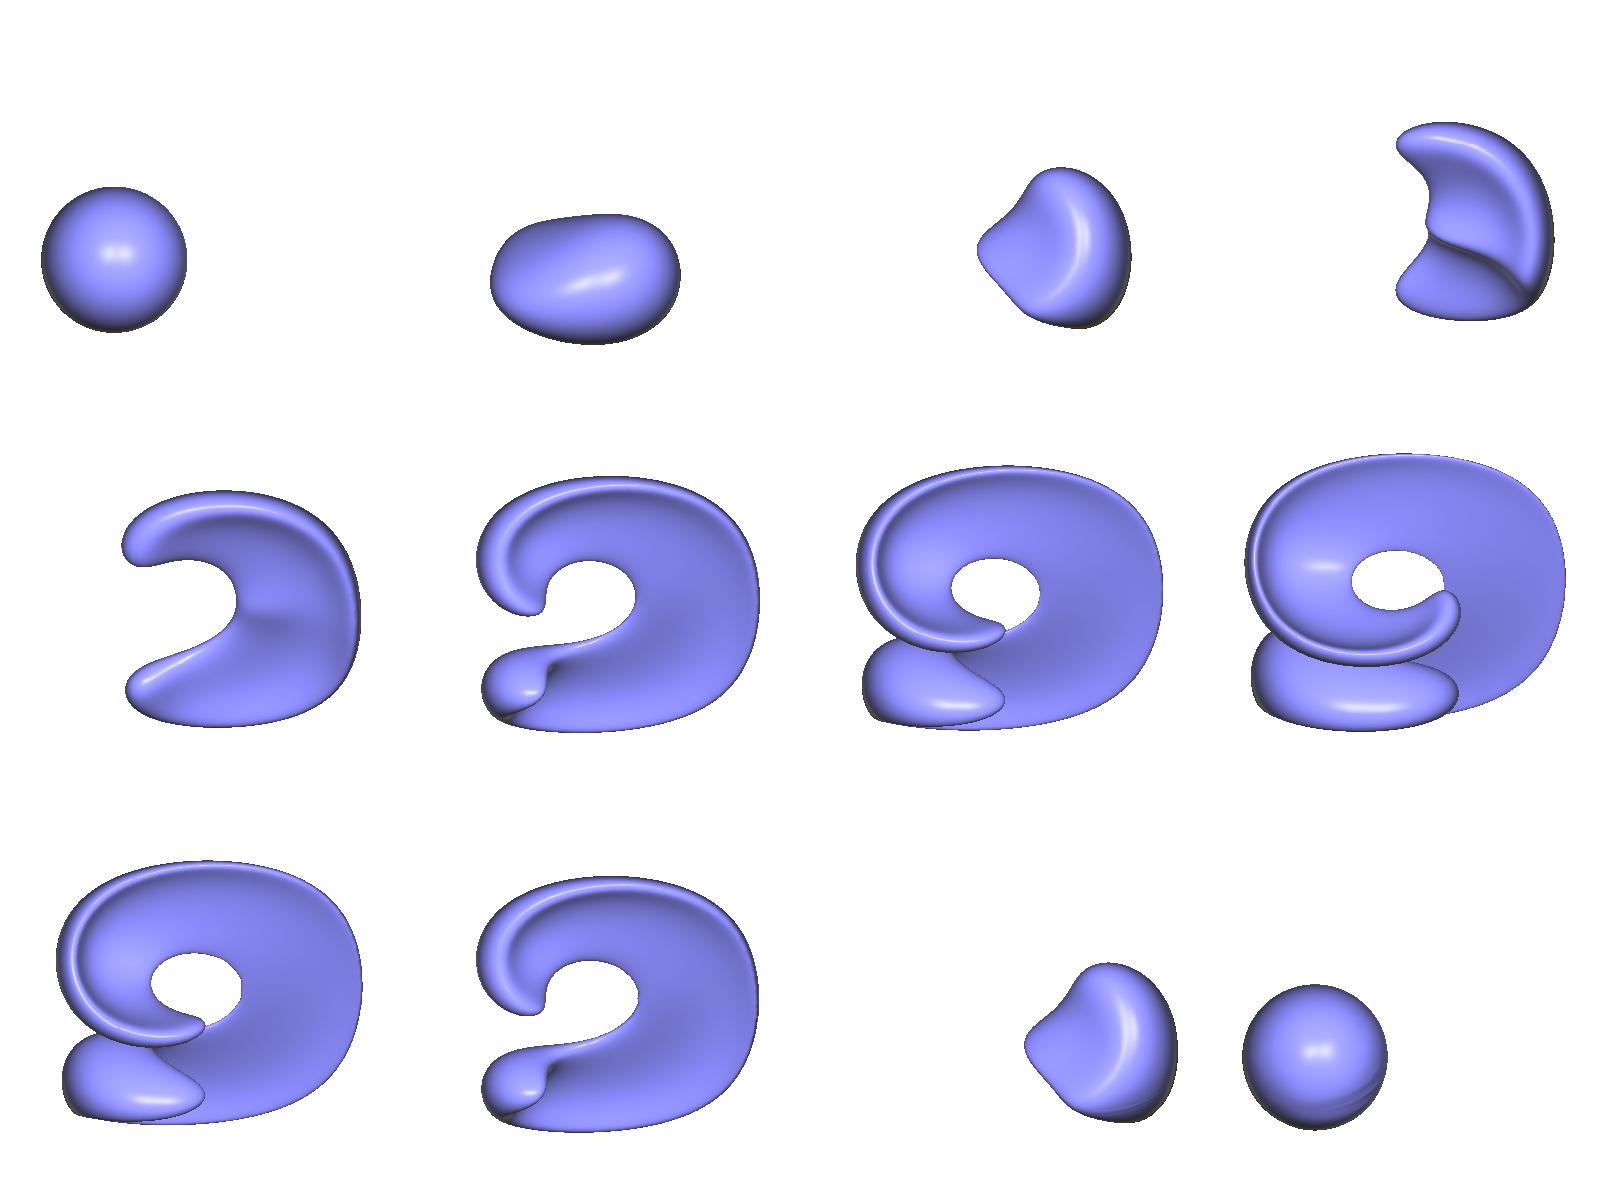
\includegraphics[scale=0.3]{enrights_test_512_until_1.eps}
\end{center}
\caption{Evolution of the interface for the Enright's test with finest resolution of $512^3$.}
\label{fig_enrights_test_until_one}
\end{figure}

\begin{figure}
\begin{center}
\includegraphics[scale=0.3]{image_0001_resolution_128.eps}\includegraphics[scale=0.3]{image_0001_resolution_256.eps}\includegraphics[scale=0.3]{image_0001_resolution_512.eps}\\
\includegraphics[scale=0.3]{image_0002_resolution_128.eps}\includegraphics[scale=0.3]{image_0002_resolution_256.eps}\includegraphics[scale=0.3]{image_0002_resolution_512.eps}\\
\end{center}
\caption{Effect of refinement on the Enright's test: The top figures correspond to the interface
fully stretched and the bottom figures correspond to the interface rewinded to the original sphere.
The finest resolutions are $128^3$ (left), $256^3$ (center) and $512^3$ (right).}
\label{fig_enrights_test_refinement}
\end{figure}

%-------------------------------------------------------------------------------
%
% Moving Interface with Curvature Dependent Speed
%
%-------------------------------------------------------------------------------
\section{Motion in the Normal Direction and Curvature Driven Flow}
The equation describing an interface propagating in its normal direction and under its mean
curvature is given by \cite{osher:1988:originallevelset}:
\begin{equation}
\phi_t+(\alpha-\beta\kappa)|\nabla\phi|=0, \label{Motion_Normal_Curvature}
\end{equation}
where $\kappa$ is the mean curvature of the interface $\kappa=\nabla\cdot\left(
\nabla\phi/|\nabla\phi| \right)$. The coefficients $\alpha$ and $\beta\ge0$ control the magnitude
of the speed in the normal direction and the strength of the curvature dependence, respectively.
The case where $\beta<0$ is ill-posed and therefore we do not consider it here.

\subsection{Motion in the Normal Direction}
First, we discuss the case when $\beta=0$. Using the second order one-sided derivatives described
in section \ref{sec_finite_differences} and discretizing the Hamiltonian using a Godunov scheme, we
semi-discretize the equation as :
$$\frac{d\phi}{dt} + \alpha\cdot H_G(\phi)=0$$
where the Godunov Hamiltonian $H_G$ is defined as:
$$H_G(\phi) =
\begin{cases}
\sqrt{\max(|(D_x^+\phi)^-|^2,|(D_x^-\phi)^+|^2)+\max(|(D_y^+\phi)^-|^2,|(D_y^-\phi)^+|^2)}&\text{if $\alpha>0$}\\
\sqrt{\max(|(D_x^+\phi)^+|^2,|(D_x^-\phi)^-|^2)+\max(|(D_y^+\phi)^+|^2,|(D_y^-\phi)^-|^2)}&\text{otherwise}
\end{cases}$$
This equation is discretized in time using the second order TVD Runge-Kutta method (see
\cite{Shu:1988:ENO,liu:1996:WENO}):
\begin{align}
\frac{\tilde{\phi}^{n+1}-       \phi ^n}{\triangle t} &+ \alpha\cdot H_G\left(\phi^n\right)=0 \\
\frac{\tilde{\phi}^{n+2}-\tilde{\phi}^n}{\triangle t} &+ \alpha\cdot H_G\left(\tilde{\phi}^{n+1}\right)=0 \\
\phi^{n+1}&=\frac{\phi^n+\tilde{\phi}^{n+2}}2
\end{align}

Table \ref{tab_shrinking_circle} illustrates that the method described above is second order
accurate in both the maximum and the average norms for smooth data. In the case where the interface
presents sharp corners, figure \ref{fig_shrinking_and_expading_square} illustrates that the method
converges to the correct viscosity solution \cite{osher:1988:originallevelset}.

\begin{table}
\begin{center}
\begin{tabular}{|c|c|c|c|c|c|c|c|}\hline
\multirow{2}{*}{} & \multicolumn{7}{|c|}{Finest Resolution}\\\cline{2-8}
                  & $64^2$ & rate & $128^2$ & rate & $256^2$ &rate & $512^2$ \\\hline
$L_1$      error of
$\phi$&$1.46\TT{-3}$&2.02&$3.58\TT{-4}$&2.00&$8.56\TT{-4}$&1.98&$2.26\TT{-5}$\\\hline $L_\infty$
error of $\phi$&$2.77\TT{-3}$&2.04&$6.72\TT{-4}$&1.95&$1.73\TT{-4}$&1.99&$4.36\TT{-5}$\\\hline
\end{tabular}
\end{center}
\caption{Convergence rate for a circle shrinking with unit normal velocity. consider a domain of
$[-2,2]^2$ and an interface initially described by a circle centered at the origin with radius
$R=1$. The interface is evolved until $t=0.5$.} \label{tab_shrinking_circle}
\end{table}
\begin{figure}
\begin{center}
\includegraphics[scale=0.5]{initial_square_new.eps}
\includegraphics[scale=0.5]{shrinking_square_point_5.eps}
\includegraphics[scale=0.5]{shrinking_square_1.eps}\\
\includegraphics[scale=0.5]{initial_square_new.eps}
\includegraphics[scale=0.5]{expanding_square_point_5.eps}
\includegraphics[scale=0.5]{expanding_square_1.eps}
\end{center}
\caption{Shrinking square in the first row, and expanding square in the second row}
\label{fig_shrinking_and_expading_square}
\end{figure}

\subsection{Adding Motion by Mean Curvature}
Now we discuss the case when $\beta>0$. The curvature term can be
discretized explicitly or implicitly. In the case where the curvature term
is discretized explicitly, the corresponding time step restriction of
$\Delta t \approx \Delta x^2$ is too stringent to be practical since it
would be constrained by the size of the smallest grid cell in the grid. In
\cite{Smereka:2003:Curvature}, Smereka proposed an implicit discretization
of the curvature term in the case of uniform grids: Using the following
operator splitting:
$$\kappa|\nabla\phi|=\Delta \phi -
\frac{\nabla\phi}{|\nabla\phi|}\nabla(|\nabla\phi|),$$ equation \eqref{Motion_Normal_Curvature} is
discretized as:
$$\frac{\phi^{n+1}-\phi^n}{\triangle t} +\alpha H_G(\phi^n) = \beta\Delta \phi^{n+1}
- \beta\frac{\nabla\phi^n}{|\nabla\phi^n|}\cdot\nabla(|\nabla\phi^n|).$$

In this work, we used a Backward Euler step to treat the linear term, and a
Forward Euler step for the nonlinear term. The derivatives $\Delta$ and
$\nabla$ are discretized by the central finite differences described in
section \ref{sec_finite_differences}. Discretizing implicitly the Laplacian
requires a linear system that we solve using the supra convergent method
presented in Min, Gibou and Ceniceros \cite{Min::Poisson_AMR_Second_Order}.
As noted in \cite{Smereka:2003:Curvature}, the semi-implicit discretization
on the curvature term allows for a big time step, so that the time step
restriction is that of the convection part, i.e.
\begin{equation}
\Delta t=\frac{\Delta x_{\text{smallest}}}{\alpha\cdot\text{\# dimensions}},
\end{equation} where $\text{\# dimensions}$ is the number of dimensions.

Table \ref{tab_circle_motion_by_curvature} demonstrates that the method is
first order accurate in the average norm for smooth a interface. The
deterioration in the maximum norm probably comes from the Elliptic part of
the solver, which propagates the errors from the regions where the grid
cells are coarse and unrefined to the regions where the grid cells are
refined. Figure \ref{fig_curvature_flow_in_octree} illustrates the motion
of an interface under mean curvature for the example presented in
\cite{Smereka:2003:Curvature}.

%So it is a first order discretization. One can go further for a better accuracy. However there is
%the following issue in this discretization. $\phi^{n+1}$ is calculated by solving a Poisson-type
%equation. As discussed in \cite{Min::Poisson_AMR_Second_Order}, the Poisson solver is second order
%accurate with the uniform refinement, i.e. splitting every cell. In level set method, it is natural
%to put the most resource near interface. So that in solving the Poisson-type equation, the errors
%in the coarse grids, i.e. the region far away from interface contaminates the region near
%interface, since the solution of one point affects the whole domain in Poisson equation. The
%accuracy of the Poisson solver in \cite{Min::Poisson_AMR_Second_Order} has not been analyzed in the
%adaptive refinement.



%\begin{figure}
%\begin{center}
%\includegraphics[scale=0.25]{curvature_flow_quadtree.eps}
%\end{center}
%\caption{$\alpha=1,\beta=1$ in $256^3$ resolution. From top-left to bottom-right, the times are $0$, $0.039$, %$0.107$, $0.507$, $0.800$ and $1.03$. The CFL condition is $\Delta t=\frac{\Delta x_{\text{smallest}}}2$. %Note that the velocities of convection and curvature cancel out not to move the side parts of the two circles %for some small time. }
%\label{fig_curvature_flow_in_quadtree}
%\end{figure}

\begin{table}
\begin{center}
\begin{tabular}{|c|c|c|c|c|c|c|c|}\hline
\multirow{2}{*}{} & \multicolumn{7}{|c|}{Finest Resolution}\\\cline{2-8}
                  & $128^2$ & rate & $256^2$ &rate & $512^2$ & rate &$1024^2$ \\\hline
$L_1$      error of $\phi$&$5.22\TT{-3}$&1.00&$2.60\TT{-3}$&0.96&$1.33\TT{-3}$&0.95&$6.95\TT{-4}$\\\hline
$L_\infty$ error of $\phi$&$5.47\TT{-3}$&0.93&$2.86\TT{-3}$&0.86&$1.56\TT{-3}$&0.81&$8.91\TT{-4}$\\\hline
\end{tabular}
\end{center}
\caption{Convergence rate for a circle with curvature dependent speed of
$\alpha=1.5$ and $\beta=1$. Initially circle is centered at $(0,0)$ with
radius one in a domain of $[-2,2]^2$. Test was run until $0.5$.The radius
$r(t)$ of the circle satisfies $r'=\alpha-\frac\beta{r}$ with $r(0)=1$.
$r(0.5)$ is approximated as $1.3108122$ from the ordinary differential
equation within error bound of $10^{-7}$.}
\label{tab_circle_motion_by_curvature}
\end{table}

%\begin{figure}
%\begin{center}
%\includegraphics[scale=0.25]{curvature_flow_quadtree.eps}
%\end{center}
%\caption{$\alpha=1,\beta=1$ in $256^3$ resolution. From top-left to
%bottom-right, the times are $0$, $0.039$, $0.107$, $0.507$, $0.800$ and
%$1.03$. The time step restriction is $\Delta t=\Delta
%x_{\text{smallest}}/2$. Note that the velocities of convection and
%curvature cancel out not to move the side parts of the two circles for some
%small time. } \label{fig_curvature_flow_in_quadtree}
%\end{figure}

\begin{figure}
\begin{center}
\includegraphics[scale=0.25]{curvature_flow_in_octree.eps}
\end{center}
\caption{Motion with curvature flow for a barbel shape. $\alpha=0,\beta=1$ in $256^3$ resolution. From top-left to bottom-right, the times are $0$, $0.023$, $0.093$, $0.140$, $0.304$ and $0.323$. The CFL condition is $\Delta t=\Delta x_{\text{smallest}}$.}
\label{fig_curvature_flow_in_octree}
\end{figure}


%--------------------------------------------------------------------------
%
%
%
%--------------------------------------------------------------------------
\section{Adaptive Grid Generation}
As the interface deforms some provisions must be given to refine the grid
near the interface while coarsening in regions farther away. The grid is
constructed in such a way that the smallest grid cells lie on the interface
as described in section \ref{sec_spatial_discretization}. This construction
depends on an input function,
$\tilde{\phi}^{n+1}:\mathbb{R}^n\to\mathbb{R}$ that is close to the signed
distance function at any point in space. This function can be constructed
in two different ways: (1) In the case where semi-Lagrangian methods are
used, a function $\tilde{\phi}^{n+1}$ can be defined as
$\tilde{\phi}^{n+1}=\phi^n(x_d)$, where $x_d$ is found by tracing back the
characteristic curves and where $\phi^n(x_d)$ is interpolated from the node
values of $\phi^n$ as described in section \ref{sec_semi_lagrangian}. (2)
In the case where the velocity field is nonlinear, semi-Lagrangian methods
cannot be used. In this case the level set function is first evolved from
$\phi^{n}$ to $\phi^{n+1}$ on the same grid $G^n$. Then $\phi^{n+1}$ is
reinitialized into a signed distance function using the algorithm described
in section \ref{sec_reinitialization}. Now at every point in space, we can
define $\tilde{\phi}^{n+1}:\mathbb{R}^n\to\mathbb{R}$ by interpolation of
$\phi^{n+1}$. Once the function
$\tilde{\phi}^{n+1}:\mathbb{R}^n\to\mathbb{R}$ can be define anywhere in
space, the new grid $G^{n+1}$ is generated by simply splitting a cell if
the Lipschitz condition: $$\min_{v\in \textrm{vertices}(C)}|\phi(v)| \le
\textrm{Lip}(\phi)\cdot \textrm{diag-size}(C)$$ is satisfied. In practice,
instead of generating $G^{n+1}$ from the root cell, we start from $G^n$ and
apply the procedure detailed in Algorithm 1, i.e. starting the recursion
from the root cell of $G^{n+1}$, the cell is recursively split if the
refinement criteria is satisfied, otherwise all of its children are merged.

\begin{center}
\begin{tabular}{ll}\hline
\multicolumn{2}{c}{\textbf{Algorithm 1} : Grid Generation} \bigstrut\\\hline
\multicolumn{2}{l}{\textbf{Input} : $G^n$ and ${\tilde{\phi}}^{n+1}:\mathbb{R}^d \to \mathbb{R}$
}\bigstrut\\\hline
1. &$G^{n+1}=G^{n}$ \\
2. &$C= \text{the root cell of } G^{n+1}$ \\
3. &\textbf{if} the Lipschitz condition for  ${\tilde{\phi}}^{n+1}$ is satisfied at $C$ \\
4. &\qquad \textbf{if} $C$ is a leaf cell \\
5. &\qquad\qquad split $C$ \\
6. &\qquad \textbf{end if} \\
7. &\qquad \textbf{for} each child cell $C'$ of $C$ \\
8. &\qquad \qquad \textbf{go to} 3 with $C=C'$ \\
9. &\qquad \textbf{end for} \\
10.&\textbf{else} \\
11.&\qquad merge $C$ \\
12.& \textbf{end if} \\\hline
\multicolumn{2}{l}{\textbf{Output} : $G^{n+1}$}\bigstrut\\\hline
\end{tabular}
\end{center}

%-------------------------------------------------------------------------------
%
% Extrapolation
%
%-------------------------------------------------------------------------------
\section{High Order Extrapolation in the Normal Direction}
The ghost fluid method, introduced by Fedkiw \etal \cite{Fedkiw:1999:ANE}, is a technique for
imposing boundary conditions at the interface in a level set framework and has been successfully
applied to a wide range of applications (see e.g.
\cite{fedkiw:2001:VSO,fedkiw:2002:CEF,Fedkiw:Ghost_Fluid:Godunov_Methods,nguyen:2001:jcpflame,
Nguyen:2002:Conservative_Ghost_Fluid,Caiden:Incompressible_Compressible,Liu:2000:ABC,Gibou:2002:Second_Order_Accurate,Gibou:2003:Crystal_Growth_JSC,
Gibou:2003:Fourth_Order_Accurate,Gibou::Vaporization} and the references therein). One basic
component of this method is the extrapolation of some scalar quantities in the normal direction. In
some cases (see e.g. \cite{Gibou:2003:Fourth_Order_Accurate}), high order extrapolations in the
normal direction are needed. This can be performed in a series of steps, as proposed in Aslam
\cite{Aslam:Extrapolation}. For example, suppose that we seek to extrapolate $u$ quadratically from
the region where $\phi\leq 0$ to the region where $\phi>0$. We first compute
$u_{nn}=\vec{n}\cdot\nabla\left( \vec{n}\cdot\nabla u \right)$ in the region where $\phi \leq 0$
and extrapolate (constant extrapolation) this quantity across the interface by solving the
following partial differential equation:
\begin{equation*}
\frac{\partial u_{nn}}{\partial \tau} + H(\phi,u_{nn})(\vec{n}\cdot\nabla u_{nn}       )=0,
\end{equation*}
where $H(\phi,u_{nn})$ is the Heaviside function defined below and $\tau$ is the fictitious time
step. Then we define $u_n$ in the region where $\phi>0$ in such a way its normal derivative is
$u_{nn}$. This can be accomplished by solving the following PDE:
\begin{equation*}
\frac{\partial u_{n }}{\partial \tau} + H(\phi,u_n)(\vec{n}\cdot\nabla u_{n }-u_{nn})=0.
\end{equation*}
Finally we can define $u$ in such a way its normal derivative is $u_n$ by solving:
\begin{equation*}
\frac{\partial u_{  }}{\partial \tau} + H(\phi,u)(\vec{n}\cdot\nabla u     -u_{n })=0.
\end{equation*}
Numerically the Heaviside function $H(\phi,S)(v_i)$ associated with a quantity $S$ at the node
$v_i$ is set to zero if the nodes involved in the computation of $S$ are all in the region where
$\phi<0$. Otherwise, it is set to 1. Therefore we define the Heaviside functions $H(\phi,u)$,
$H(\phi,u_{n})$ and $H(\phi,u_{nn})$ as follows:
\begin{align*}
H(\phi,u)(v_i) &= \begin{cases}
                 0 & \text{ if $\phi(v_i)<0$ } \\
                 1 & \text{ otherwise}
                 \end{cases} ,\\
H(\phi,u_n)(v_i) &= \begin{cases}
                   0 & \text{ if $H(\phi,u)(v_j)=0$ for all $v_j\in$ ngbd$(v_i)$} \\
                   1 & \text{ otherwise}
                   \end{cases} ,\\
H(\phi,u_{nn})(v_i) &= \begin{cases}
                   0 & \text{ if $H(\phi,u_n)(v_j)=0$ for all $v_j\in$ ngbd$(v_i)$} \\
                   1 & \text{ otherwise}
                   \end{cases},
\end{align*}
where $\text{ngbd}(v_i)$ denotes the set of direct neighboring nodes of $v_i$. The quantity
$u_n=\vec{n}\cdot\nabla u$ is computed by the central finite differences described in section
\ref{sec_finite_differences} for all the nodes where $H(\phi,u_n)=0$. Likewise, using the values of
$u_{nn}$ is then computed by central differencing for all the nodes where $H(\phi,u_{nn})=0$. The
three partial differential equations above are discretized in a dimension by dimension framework
using the upwind schemes and the one-sided finite differences of section
\ref{sec_finite_differences}, i.e. the discretizations in a semi-discrete form read:
\begin{align*}
\frac{d}{d\tau}u_{nn}+H(\phi,u_{nn})\left(n_x^+D_x^-u_{nn}+n_x^-D_x^+u_{nn}\right)&=0,
\end{align*}
\begin{align*}
\frac{d}{d\tau}u_{n }+H(\phi,u_{n })\left(n_x^+D_x^-u_{n }+n_x^-D_x^+u_{n }\right)&=H(\phi,u_{n})
u_{nn},
\end{align*}
and
\begin{align*}
\frac{d}{d\tau}u     +H(\phi,u     )\left(n_x^+D_x^-u     + n_x^-D_x^+u    \right)&=H(\phi,u ) u_{n
}.
\end{align*}
These semi-discrete equations are then evolved in time using the same TVD RK-2 method of section
\ref{sec_reinitialization}. Since the equations are evolved in fictitious time, we can take the
same time step restriction as in the reinitialization procedure of section
\ref{sec_reinitialization}.

Figure \ref{extrapolation_aslam} illustrates the constant, linear and quadratic extrapolation
obtained with the algorithm described above: Consider a computational domain $\Omega=(-\pi,
\pi)\times(-\pi, \pi)$ separated into two regions: $\Omega^-$ defined as the interior of a disk
with center at the origin and radius two, and $\Omega^+=\Omega \setminus \Omega^-$. The function
$u$ to be extrapolated from $\Omega^-$ to $\Omega^+$ is defined as $u=\cos(x)\sin(y)$ for $x \in
\Omega^-$. We have extrapolated $u$ in the entire region in this example for the sake of
presentation but we emphasize that in practice the extrapolation is performed only in a
neighborhood of the interface. Tables \ref{table_constant_extrapolation},
\ref{table_linear_extrapolation} and \ref{table_quadratic_extrapolation} demonstrate the first
order accuracy for the constant extrapolation, the second order accuracy for the linear
extrapolation and the third order accuracy for the quadratic extrapolation. We note that it is
enough to discretize $D^{\pm}_xu_{nn}$ and $D^{\pm}_xu_{n}$ with the first order accurate finite
difference of section \ref{sec_finite_differences}, and $D^{\pm}_xu$ with the second order accurate
finite difference in section \ref{sec_finite_differences} to achieve third order accuracy in $u$ in
the case of a quadratic extrapolation. The same accuracy would be achieved in the case where the
second order accurate finite differences were used for $D^{\pm}_xu_{nn}$, $D^{\pm}_xu_{n}$, and
$D^{\pm}_xu_{n}$. However, using the first order accurate finite difference schemes for
$D^{\pm}_xu_{nn}$ and $D^{\pm}_xu_{n}$ yields more robust results since $u_{nn}$ and $u_{n}$ may be
noisy unless $u$ is a very smooth function.


\begin{table}
\begin{center}
\begin{tabular}{|c|c|c|c|c|c|c|}
\hline Finest &$L^\infty$ error&rate&$L^1 error$&rate \\ Resolution& of $\phi$      &    & of
$\phi$ & \\\hline

$32^2$&$5.11\times10^{-1}$& &$1.11\times10^{-1}$&      \\\hline
$64^2$&$2.55\times10^{-1}$&1.01&$3.75\times10^{-2}$&1.56   \\\hline
$128^2$&$1.25\times10^{-1}$&1.02&$1.06\times10^{-2}$&1.82   \\\hline
$256^2$&$6.20\times10^{-2}$&1.01&$2.89\times10^{-3}$&1.87   \\\hline
$512^2$&$3.14\times10^{-2}$&.97&$7.59\times10^{-4}$&1.92   \\\hline
$1024^2$&$1.59\times10^{-2}$&.98&$2.01\times10^{-4}$&1.91   \\\hline
\end{tabular}
\end{center}
\caption{Convergence rate for the constant
extrapolation}\label{table_constant_extrapolation}
\end{table}

\begin{table}
\begin{center}
\begin{tabular}{|c|c|c|c|c|c|c|}
\hline Effective &$L^\infty$ error&rate&$L^1 error$&rate \\ Resolution& of $\phi$      &    & of
$\phi$ & \\\hline

$32^2$&$2.02\times10^{-1}$& &$3.52\times10^{-2}$&      \\\hline
$64^2$&$7.21\times10^{-2}$&1.48&$6.09\times10^{-3}$&2.53   \\\hline
$128^2$&$1.78\times10^{-2}$&2.00&$8.79\times10^{-4}$&2.79   \\\hline
$256^2$&$5.27\times10^{-3}$&1.76&$1.19\times10^{-4}$&2.88   \\\hline
$512^2$&$1.12\times10^{-3}$&2.22&$1.54\times10^{-5}$&2.94   \\\hline
$1024^2$&$2.83\times10^{-4}$&1.99&$2.04\times10^{-6}$&2.91   \\\hline
\end{tabular}
\end{center}
\caption{Convergence rate for the linear
extrapolation}\label{table_linear_extrapolation}
\end{table}


\begin{table}
\begin{center}
\begin{tabular}{|c|c|c|c|c|c|c|}
\hline Effective &$L^\infty$ error&rate&$L^1 error$&rate \\ Resolution& of $\phi$      &    & of
$\phi$ & \\\hline

$32^2$&$1.62\times10^{-1}$& &$2.26\times10^{-2}$&      \\\hline
$64^2$&$2.31\times10^{-2}$&2.82&$2.21\times10^{-3}$&3.36   \\\hline
$128^2$&$2.95\times10^{-3}$&2.96&$1.65\times10^{-4}$&3.73   \\\hline
$256^2$&$3.81\times10^{-4}$&2.95&$1.17\times10^{-5}$&3.81   \\\hline
$512^2$&$4.89\times10^{-5}$&2.96&$7.82\times10^{-7}$&3.91   \\\hline
$1024^2$&$6.19\times10^{-6}$&2.98&$5.31\times10^{-8}$&3.88   \\\hline
\end{tabular}
\end{center}
\caption{Convergence rate for the quadratic
extrapolation}\label{table_quadratic_extrapolation}
\end{table}

\begin{figure}
\begin{center}
\includegraphics[scale=0.25]{constant_extrapolation.eps}\includegraphics[scale=0.25]{linear_extrapolation.eps}\includegraphics[scale=0.25]{quadratic_extrapolation.eps}
\includegraphics[scale=0.2]{constant_extrapolation_zoom.eps}\hspace{1cm}\includegraphics[scale=0.2]{linear_extrapolation_zoom.eps}\hspace{1cm}\includegraphics[scale=0.2]{quadratic_extrapolation_zoom.eps}
\end{center}
\caption{Contours of the solution after it has been extrapolated across the
interface with a constant (left), linear (center) and quadratic (right)
extrapolations across an interface. The top row illustrates the
extrapolation on the entire domain and the bottom row is a zoom near the
interface. The exact solution is given inside the circle centered at the
origin and with radius 2 and is extrapolated outside in the normal
direction. We then plot the level curves of the solution.}
\label{extrapolation_aslam}
\end{figure}


\section{Conclusion}
We have presented a level set method on non-graded adaptive Cartesian
grids, i.e. grids for which the ratio between adjacent cells is not
constrained. We use quadtree and octree data structures to represent the
grid and a simple algorithm to generate a mesh with the finest resolution
at the interface. We have presented (1) a locally third order accurate
reinitialization scheme that transforms an arbitrary level set function
into a signed distance function, (2) a second order accurate
semi-Lagrangian methods to evolve the linear level set advection equation
under an externally generated velocity field, (3) a second order accurate
upwind method to evolve the nonlinear level set equation under a normal
velocity as well as to extrapolate scalar quantities across an interface in
the normal direction, and (4) a semi-implicit scheme to evolve the
interface under mean curvature. This method produces results with a
negligible amount of mass loss. We have proposed numerical examples in two
and three spatial dimensions to demonstrate the accuracy of the method.

\section{Acknowledgment}
The research of F. Gibou was supported in part by the Alfred P. Sloan Foundation through a research
fellowship in Mathematics.
%-------------------------------------------------------------------------------
%
% References : "reference.bib"
%
%-------------------------------------------------------------------------------
\bibliographystyle{plain}
\addcontentsline{toc}{section}{\refname}\bibliography{../references}


\end{document}
